% !TEX program = xelatex
\documentclass[a4paper]{article}
\usepackage{amsmath}
\usepackage{amsthm}
\usepackage[left=1.8cm,right=1.8cm,top=2.2cm,bottom=2.0cm]{geometry}
\usepackage{ctex}
\usepackage{enumerate}
\usepackage{fancyhdr}
\usepackage{xpatch}
\usepackage{graphicx} 
\usepackage{float} 
\usepackage{subfigure} 
\usepackage{amsfonts}
\usepackage{mathtools}
\usepackage{framed}
\usepackage{multicol}
\usepackage{listings,listings-rust}
\usepackage{hyperref}
\usepackage{tikz}
\usetikzlibrary{automata,positioning}
\theoremstyle{definition}
\newtheorem*{solution*}{\textbf{Solution:}}
\newtheorem*{proof*}{\textbf{Proof:}}
\newtheorem{theorem}{Theorem}[subsection]
\newtheorem{definition}{Definition}[subsection]
\newtheorem{lemma}{Lemma}[subsection]
\makeatletter
% \usepackage{listings}% http://ctan.org/pkg/listings
\lstset{
  basicstyle=\ttfamily\tiny,
  mathescape,
}
\AtBeginDocument{\xpatchcmd{\@thm}{\thm@headpunct{.}}{\thm@headpunct{}}{}{}}
\makeatother

\pagestyle{fancy}
\renewcommand{\baselinestretch}{1.15}

\usepackage{paralist}
\let\itemize\compactitem
\let\enditemize\endcompactitem
\let\enumerate\compactenum
\let\endenumerate\endcompactenum
\let\description\compactdesc
\let\enddescription\endcompactdesc

% shorten footnote rule
\xpatchcmd\footnoterule
  {.4\columnwidth}
  {1in}
  {}{\fail}
  \pagestyle{fancy}
  \renewcommand{\baselinestretch}{1.15}
  \usepackage[scaled=0.85]{FiraMono}
  
  \lstset{basicstyle=\ttfamily, keywordstyle=\bfseries}
\title{CS 131 Compilers: Discussion 11: Operational Semantic and Runtime Resourse Allocation}
\author{\textbf{杨易为}~~\textbf{季杨彪}~~\textbf{尤存翰} \\ \texttt{ \{yangyw,jiyb,youch\}@shanghaitech.edu.cn}}


\begin{document}
\maketitle

\section{Type System Cont.}
\subsection{Last time}

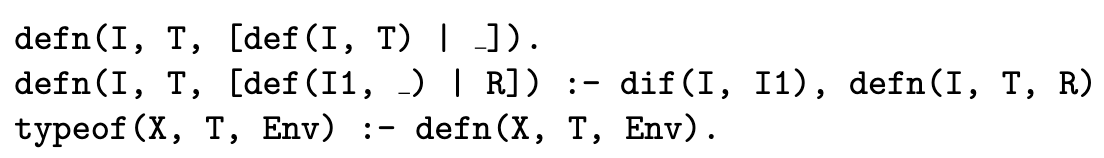
\includegraphics[width=10cm]{img/Snipaste_2021-05-17_17-48-16.png}

\subsection{Type Inference in Rust/C++}
Rust is a good language to do type inference utilizing the trait. Type inference is the process of automatic detection of the type of an expression.

\begin{lstlisting}[language=Rust]
fn main() {
    let mut things = vec![];
    things.push("thing");
}
\end{lstlisting}
Here, the type of $things$ is inferred to be $Vec<\&str>$ because of the value we push into $things$.

The type inference is based on the standard Hindley-Milner (HM) type inference algorithm. 

Before C++20, we may find it difficult to write good type inference in Generic Type. For example

\begin{lstlisting}[language=C]
template<typename T> T add(T in1, T in2) {
    return in1 + in2;
}
class Complex {
public:
    double real = 0;
    double imaginary = 0;
};
\end{lstlisting}
The compiler will emit such error: 
\begin{enumerate}
  \item no match for 'operator+' (operand types are 'Complex' and 'Complex')
  \item 'Complex' is not derived from 'const std::cxx11::basic\_string<\_CharT, \_Traits, \_Allocator>' \dots
  \item mismatched types 'const\_CharT*' and 'Complex'
\end{enumerate}
Since this template function is already available for integers and double precision numbers, the cause of the error is not in the template function itself, but in the call to the template using the actual data Complex. but the problem is that the error message does not indicate which call is the problem.

Also, the error message indicates that there is no matching + operator, which is the real cause. But then Complex does not inherit from various classes and other accompanying information only adds to the confusion. The authors believe that any programmer who has used generic programming will have had a similar experience.

The solution is simple: just overload the + operator for Complex

\subsection{Type Coercion}
Type coercion is the automatic or implicit conversion of values from one data type to another (such as strings to numbers). Type conversion is similar to type coercion because they both convert values from one data type to another with one key difference — type coercion is implicit whereas type conversion can be either implicit or explicit.

\begin{lstlisting}[language=C]
  // implicit conversion of classes:
  #include <iostream>
  using namespace std;
  
  class A {};
  
  class B {
  public:
    // conversion from A (constructor):
    B (const A& x) {}
    // conversion from A (assignment):
    B& operator= (const A& x) {return *this;}
    // conversion to A (type-cast operator)
    operator A() {return A();}
  };
  
  int main ()
  {
    A foo;
    B bar = foo;    // calls constructor
    bar = foo;      // calls assignment
    foo = bar;      // calls type-cast operator
    return 0;
  }
  \end{lstlisting}
\section{Operational Semantic}
Suppose we have already defined the operational semantics of basic arithmetic expressions involving the integers, variables, and booleans as follows (respectively):

$$\frac{\cdots}{\Gamma \vdash e_{1}: n, \Gamma}$$
and
$$\frac{\cdots}{\Gamma \vdash b_{1}: b, \Gamma}$$

$\Gamma$ here represents our mapping between variables and their values. We use the convention $e$ for arithemtic expressions and $b$ for boolean expressions. Note that as of now, expressions do not modify the state of our program. Write the operational semantics for the following types of constructs:

\begin{enumerate}
  \item Assignment to an arithmetic expression as follows: $x:=e$. Note an assignment returns void.
  \item A sequence of statements $s_{1}$ and $s_{2}$ as follows: $s_{1} ; s_{2} .$ Note a sequence returns void.
  \item An if statement as follows: if $b$ then $s_{1}$ else $s_{2} .$ Note an if statement must only execute its corresponding branch.
\end{enumerate}

\subsection{Runtime support for functions}
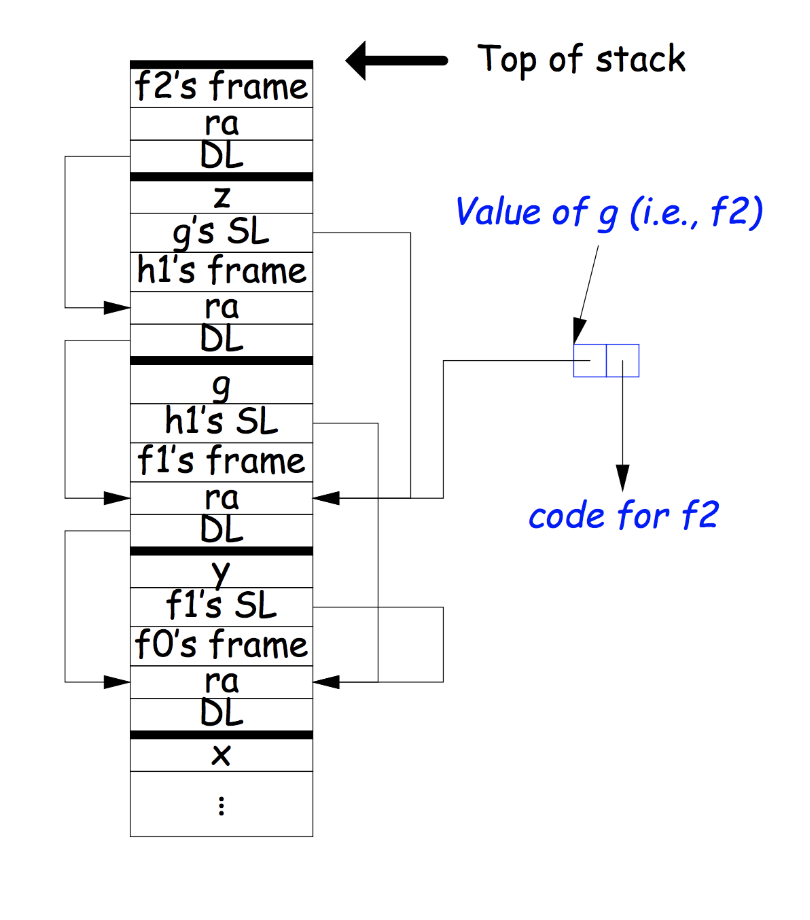
\includegraphics[width=10cm]{img/Snipaste_2021-05-17_17-51-44.png}
\end{document}
